\documentclass[a4paper, 12pt]{article}

\usepackage[top=2cm,bottom=2cm,left=3cm,right=3cm]{geometry}

\usepackage[T2A]{fontenc}
\usepackage[utf8]{inputenc}
\usepackage[english,russian]{babel}
\usepackage{indentfirst}

\usepackage{graphicx}
\usepackage{xcolor}

\usepackage{amsmath}

\usepackage[some]{background}
\usepackage{paratype}

\definecolor{titlepagecolor}{cmyk}{1,.60,0,.40}

\DeclareFixedFont{\bigsf}{T2A}{PTSans-TLF}{b}{n}{1.4cm}

\backgroundsetup{
scale=1,
angle=0,
opacity=1,
contents={\begin{tikzpicture}[remember picture,overlay]
 \path [fill=titlepagecolor] (-0.5\paperwidth,5) rectangle (0.5\paperwidth,10);  
\end{tikzpicture}}
}

\makeatletter

\def\printauthor{%                  
    {\large \@author}}              
\makeatother

\author{%
    Луговцов Глеб\\
    ФЭФМ МФТИ\\
    \texttt{lugovtsov.gs@phystech.edu}\vspace{40pt}\\
    % Author 2 name \\
    % Department name \\
    % \texttt{email2@example.com}
}

\newcommand{\artitle}{Изучение плазмы газового\\[9pt] разряда в неоне}

\newcommand{\arabstract}{В работе изучается плазма газового разряда в неоне, ВАХ разряда и описание свойств полученной плазмы с помощью некоторых параметров.}

\newcommand{\imageheight}{8cm}

\begin{document}

\begin{titlepage}
\BgThispage
\newgeometry{left=1.5cm,right=3cm}
\vspace*{2cm}
\noindent
\textcolor{white}{\bigsf \artitle}
\vspace*{2cm}\par
\noindent
\begin{minipage}{0.48\linewidth}
    \begin{flushright}
        \printauthor
    \end{flushright}
\end{minipage} \hspace{15pt}
%
\begin{minipage}{0.02\linewidth}
    \rule{1pt}{175pt}
\end{minipage} \hspace{-15pt}
%
\begin{minipage}{0.65\linewidth}
\vspace{5pt}
    \begin{abstract}
        \arabstract
    \end{abstract}
\end{minipage}
\end{titlepage}
\restoregeometry

\section{Введение}
Плазмой называют четвёртое агрегатное состояние, при котором вещество (в нашем случае это неон) диссоциирует на газ из свободных ионов, электронов и нейтральных частиц, которые не распались. Поведение этого газа можно описать множеством параметров, таких как температура, плазменная частота, радиус Дебая, среднее число ионов в дебаевской сфере. В этой работе мы постараемся подробно изучить поведение плазмы на примере двойного зонда и разряда.

\section{Теоретическая справка}

\subsection*{Плазма}
В ионизированном газе поле ионов <<экранируется>> электронами. Для поля $\mathbf{E}$ и плотности $\rho$ электрического заряда
$$
\text{div}~\mathbf{E} = 4 \pi \rho,
$$
а с учётом сферической симметрии и $\mathbf{E} = -\text{grad}~\varphi$:
\begin{equation}
    \dfrac{d^2 \varphi}{dr^2}+\dfrac{2}{r}\dfrac{d\varphi}{dr}=-4\pi \rho.
\end{equation}
Плотности заряда электронов и ионов (которые мы считаем бесконечно тяжёлыми и поэтому неподвижными)
\begin{equation}
    \begin{array}{c}
        \rho_e = -ne \cdot \exp\left(\dfrac{e\varphi}{kT_e}\right),\\
        \rho_i = ne.
    \end{array}
\end{equation}
Тогда из $(1)$ в предположении $\dfrac{e\varphi}{kT_e} \ll 1$ получим
\begin{equation}
    \varphi = \dfrac{Ze}{r}e^{-r/r_D},
\end{equation}
где $r_D = \sqrt{\dfrac{kT_e}{4\pi n e^2}}$ -- \textit{радиус Дебая}. Среднее число ионов в сфере такого радиуса 
\begin{wrapfigure}{r}{4cm}
    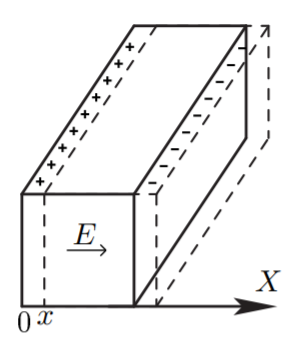
\includegraphics[scale=0.5]{images/figure.png}
    \caption{Плазменные колебания}
\end{wrapfigure}  
\begin{equation}
    N_D = n\dfrac{4}{3}\pi r_D^2.
\end{equation}
Теперь выделим параллелепипед с плотностью $n$ электронов, сместим их на $x$. Возникнут поверхностные заряды $\sigma = nex$, поле от которых будет придавать электронам ускорение:
$$
\dfrac{d^2x}{dt^2}=-\dfrac{eE}{m}=-\dfrac{4\pi n e^2}{m}x.
$$ 
Отсюда получаем \textit{плазменную (ленгмюровскую) частоту} колебаний электронов:
\begin{equation}
    \omega_p = \sqrt{\dfrac{4\pi ne^2}{m}}.
\end{equation}
\subsection*{Одиночный зонд}
При внесении в плазму уединённого проводника -- \textit{зонда} -- с потенциалом, изначально равным потенциалу точки плазмы, в которую его помещают, на него поступают токи электроннов и ионов:
\begin{equation}
    \begin{array}{c}
        I_{e0} = \dfrac{n \langle v_e \rangle}{4}eS,\\
        I_{i0} = \dfrac{n \langle v_i \rangle}{4}eS,
    \end{array}
\end{equation}
где $\langle v_e \rangle$ и $\langle v_i \rangle$ -- средние скорости электронов и ионов, $S$ -- площадь зонда, $n$ -- плотность электронов и ионов. Скорости электронов много больше скорости ионов, поэтому $I_{i0} \ll I_{e0}$. Зонд будет заряжаться до некоторого равновестного напряжения $-U_f$ -- \textit{плавающего потенциала}.\\
\begin{wrapfigure}{r}{5.5cm}
    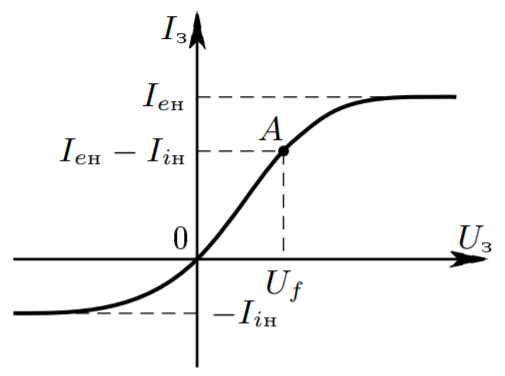
\includegraphics[scale=0.5]{images/zond.png}
    \caption{Вольт-амперная характеристика одиночного зонда}
\end{wrapfigure}  
В равновесии ионный ток мало меняется, а электронный имеет вид
$$
I_e = I_0 \exp\left( -\dfrac{eU_f}{kT_e} \right).
$$
Будем подавать потенциал $U_\text{з}$ на зонд и снимать значение зондового тока $I_\text{з}$. Максимальное значение тока $I_{e\text{н}}$ -- электронный ток насыщения, а минимальное $I_{i\text{н}}$ -- ионный ток насыщения. Значение из эмпирической формулы Бомона:
\begin{equation}
    I_{i\text{н}} = 0.4 neS \sqrt{\dfrac{2kT_e}{m_i}}.
\end{equation}
\subsection*{Двойной зонд}
Двойной зонд -- система из двух одинаковых зондов, расположенных на небольшом расстоянии друг от друга, между которыми создаётся разность потенциалов, меньшая $U_f$. Рассчитаем ток между ними вблизи $I=0$. При небольших разностях потенциалов ионные токи на оба зонда близки к току насыщения и компенсируют друг друга, а значит величина результирующего тока полностью связана с разностью электронных токов. Пусть потенциалы на зондах
$$
U_1 = -U_f + \Delta U_1,
$$
$$
U_2 = -U_f + \Delta U_2.
$$
Между зондами $U = U_2 - U_1 = \Delta U_2 - \Delta U_1$.
Через первый электрод
\begin{equation}
    I_1 = I_{i\text{н}} + I_{e1} = I_{i\text{н}} - \dfrac{1}{4}neS\langle v_e\rangle \exp\left(-\dfrac{eU_f}{kT_e}\right)\exp\left(\dfrac{e\Delta U_1}{kT_e}\right)=I_{i\text{н}}\left(1 - \exp\left( \dfrac{e\Delta U_1}{kT_e} \right)\right).
\end{equation}
Аналогично через второй получим
\begin{equation}
I_2 = I_{i\text{н}}\left(1 - \exp\left( \dfrac{e\Delta U_2}{kT_e} \right)\right)
\end{equation}
  
Из $(7)$ и $(8)$ с учётом последовательного соединение зондов ($I_1 = -I_2 = I)$:
$$
\Delta U_1= \dfrac{kT_e}{e}\text{ln}\left(1 - \dfrac{I}{I_{i\text{н}}}\right)
$$
$$
\Delta U_2= \dfrac{kT_e}{e}\text{ln}\left(1 + \dfrac{I}{I_{i\text{н}}}\right)
$$

Тогда итоговые формулы для разности потенциалов и тока

\begin{equation}
    U = \dfrac{kT_e}{e}\text{ln}\dfrac{1 - I/I_{i\text{н}}}{1 + I/I_{i\text{н}}}, 
    I = I_{i\text{н}} \text{th}\dfrac{eU}{2kT_e}.
\end{equation}
Реальная зависимость выглядит несколько иначе и описывается формулой 
\begin{wrapfigure}{l}{7cm}
    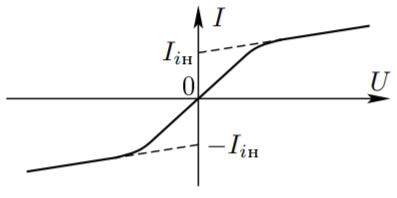
\includegraphics[scale=0.8]{images/double_zond.png}
    \caption{Вольт-амперная характеристика двойного зонда}
    \vspace{+30pt}
\end{wrapfigure}
\begin{equation}
    I = I_{i\text{н}} \text{th}\dfrac{eU}{2kT_e} + AU.
\end{equation}
Из этой формулы можно найти формулу для $T_e$: для $U=0$ мы найдём $I_{i\text{н}}$, продифференцируем в точке $U=0$ и с учётом $\text{th}~\alpha \approx \alpha$ при малых $\alpha$ и $A\rightarrow 0$ получим:
\begin{equation}
    kT_e = \dfrac{1}{2}\dfrac{eI_{i\text{н}}}{\dfrac{dI}{dU}|_{U=0}}.
\end{equation}
\\

\section{Ход работы}
\subsection*{Описание установки}

\begin{figure}[!h]
    \centering
    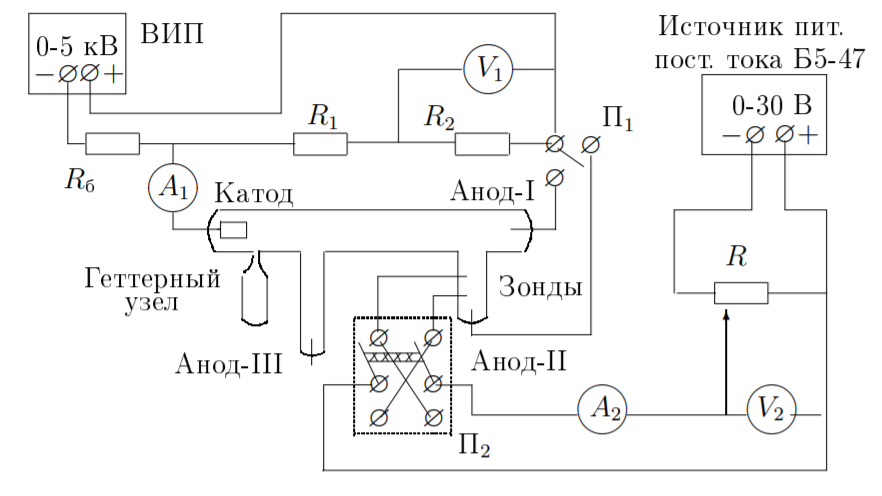
\includegraphics[scale=0.6]{images/scheme.png}
    \caption{Принципиальная схема установки}
    \label{fig:my_label}
\end{figure}

Стеклянная газоразрядная трубка имеет холодный (ненакаливаемый) полый катод, три анода и \textit{геттерный} узел -- стеклянный баллон, на внутреннюю повехность которого напылена газопоглощающая плёнка (\textit{геттер}). Трубка наполнена изотопом неона $^22$Ne при давлении 2 мм рт. ст. Катод и один из анодом (I и II) с помощью переключателя $\Pi_1$ подключается через балластный резистор $R_\text{б}$ ($\approx 450$ кОм) к регулируемому ВИП с выкодным напряжением до 5 кВ.\\
При подключении к ВИП анода-I между ним и катодом возникает газовый разряд. Ток разряда измеряется миллиамперметром $A_1$, а падение напряжения на разрядной трубке -- цифровым вольтметром $V_1$, подключённым к трубке черезе высокоомный (25 МОм) делитель напряжения с коэффициентом $(R_1+R_2)/R_2 = 10$.\\
При подключении к ВИП анода-II разряд возникает в пространстве между катодом и анодом-II, где находятся двойной зонд, используемый для диагностики плазмы положительного столба. Зонды изготовлены из молибденовой проволоки диаметром $d = 0.2$ мм и имеют длину $l = 5.2$ мм. Они подключены к источнику питания GPS через потенциометр $R$. Переключатель $\Pi_2$ позволяет изменять полярность напряжения на зондах. Величина напряжения на зондах изменяеься с помощью дискретного переключателя <<$V$>> выходного напряжения источника питания и потенциометра $R$, а измеряется цифровым вольтметром $V_2$. Для измерения зондового тока используется мультиметр $A_2$.


\subsection*{Исследование ВАХ разряда}
Зажигаем плазму и строим ВАХ разряда в координатах $I_\text{р}(U_\text{р})$:

\begin{figure}[!h]
    \centering
    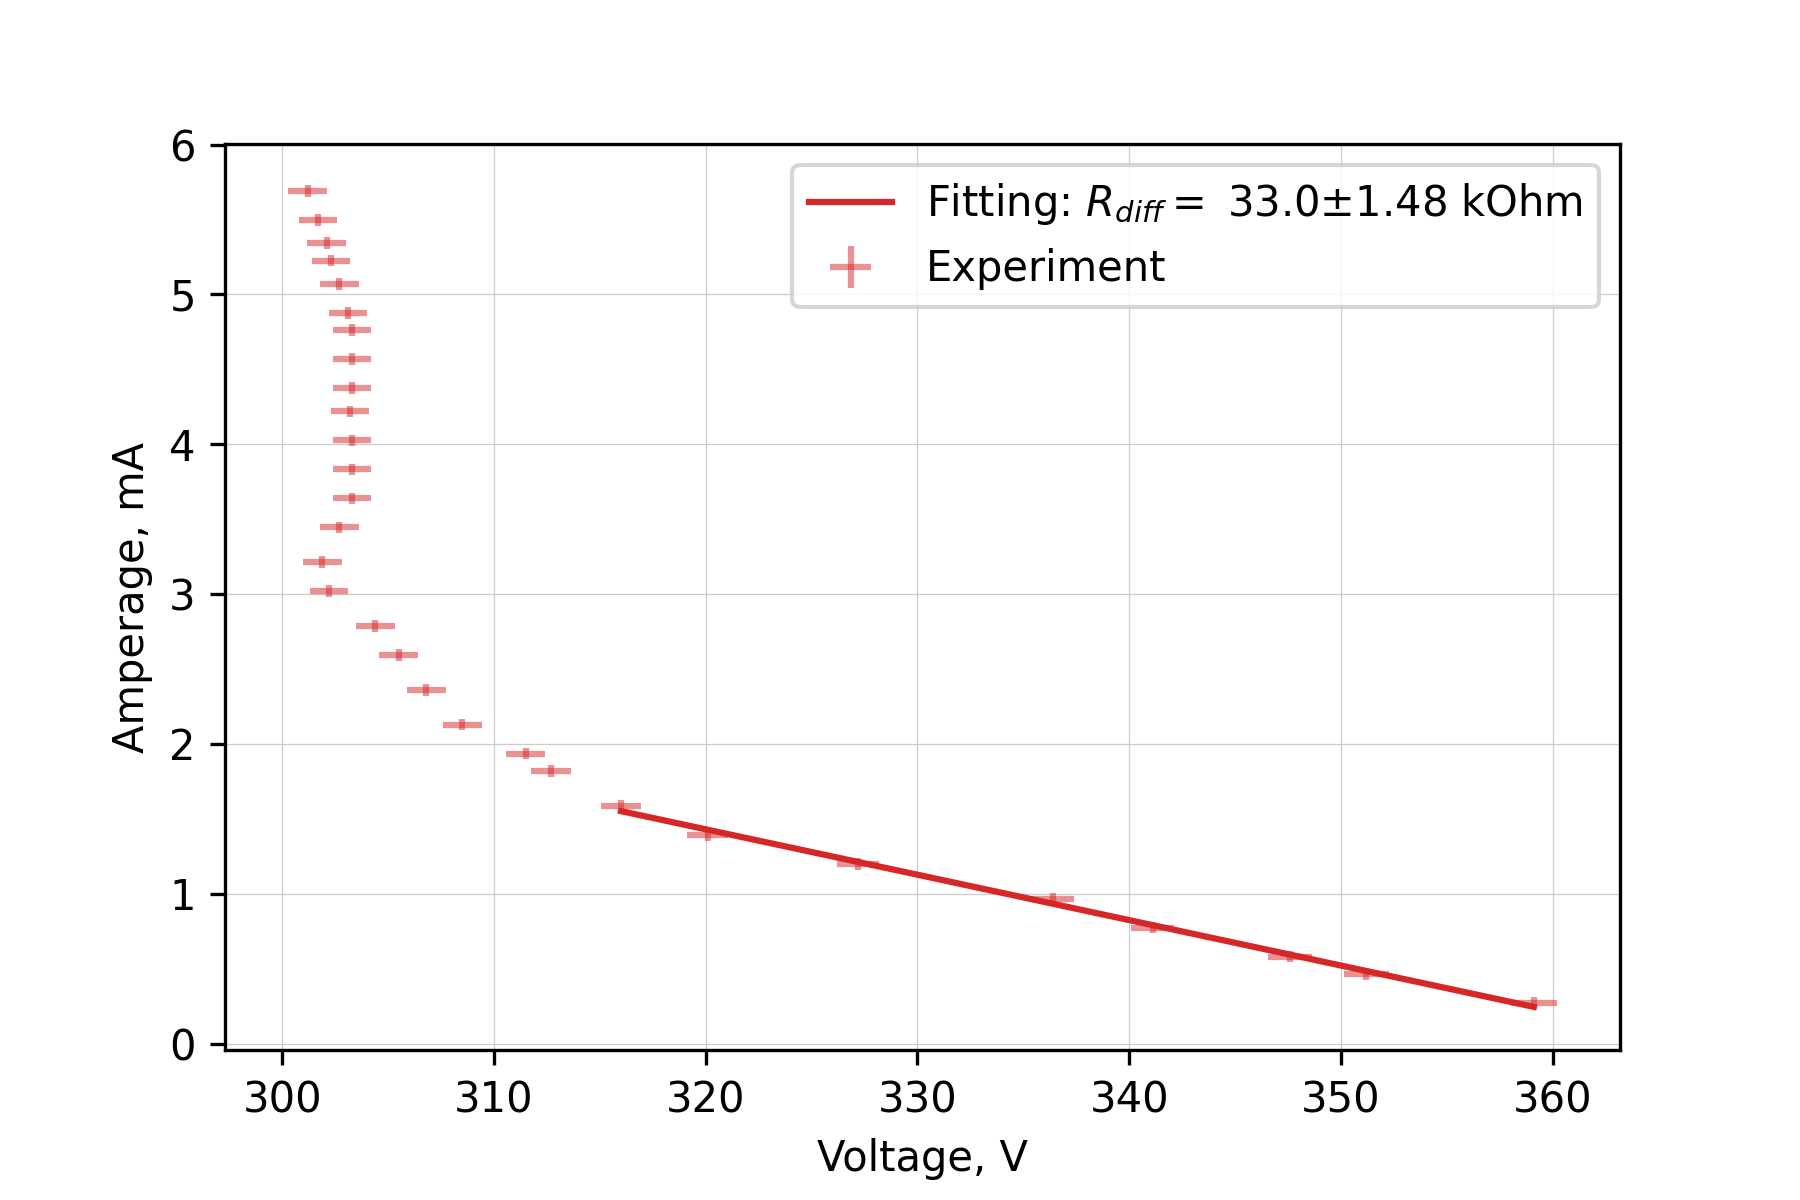
\includegraphics[height=\imageheight]{images/vah-discharge.png}
    \caption{ВАХ разряда}
    \label{fig:vah-discharge}
\end{figure}

По наклону того участка кривой, который приближен к линии, находим максимальное диффиренциальное сопротивление разряда $R_\text{диф}$ (обратный коэффициент прямой):

\begin{equation}
    R_\text{диф} = \dfrac{dU}{dI} = 33.0 \pm 1.5 \text{ кОм}
\end{equation}

Сравнивная полученную кривую с рисунком \ref{fig:vah-dis-all} мы приходим к выводу, что состояние будет называться \textit{поднормальным тлеющим зарядом} (участок ГД). Полное описание есть на стр. 283 практикума.

\begin{figure}[h]
    \centering
    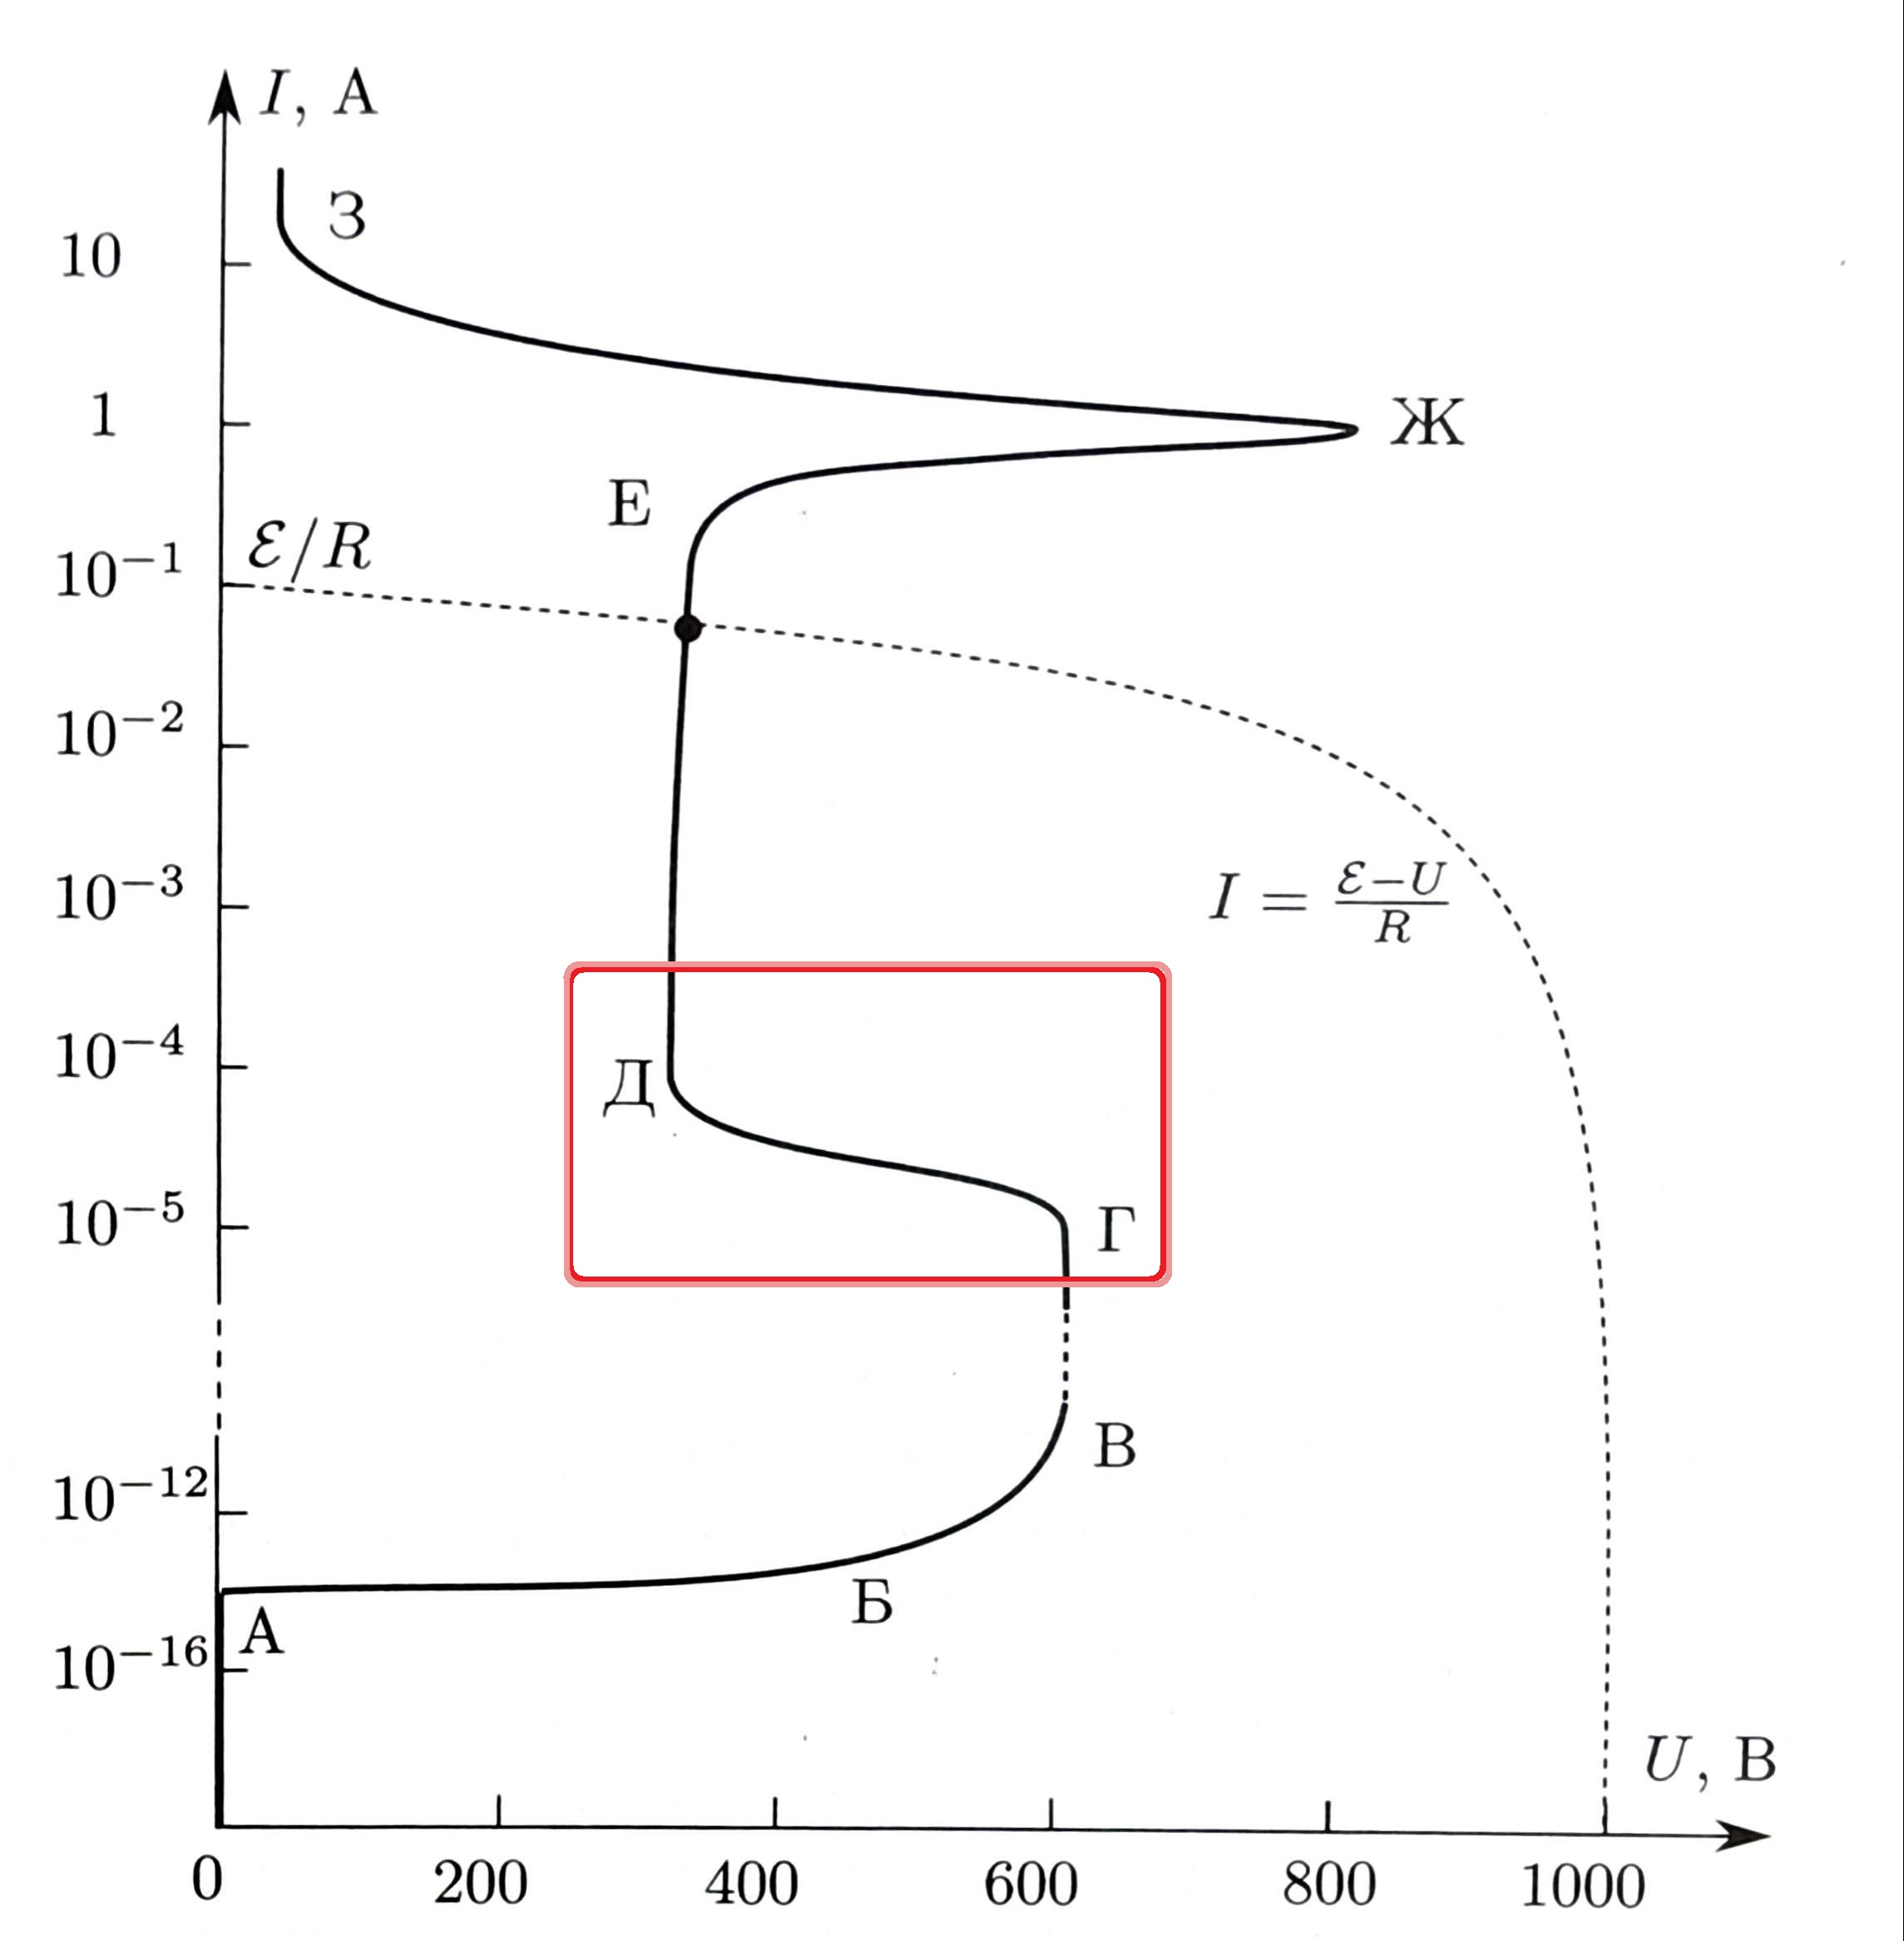
\includegraphics[height=\imageheight]{images/vah_discharge_all.jpg}
    \caption{Вольт-амперная характеристика разряда в неоне при давлении 1 торр. Пунктиром изображён пример нагрузочной прямой, соответствующей режиму нормального тлеющего разряда.}
    \label{fig:vah-dis-all}
\end{figure}

\newpage
\subsection*{Исследование зондовых характеристик}

Построим зондовые характеристики для разных токов и отцентруем кривые:

\begin{figure}[!h]
    \centering
    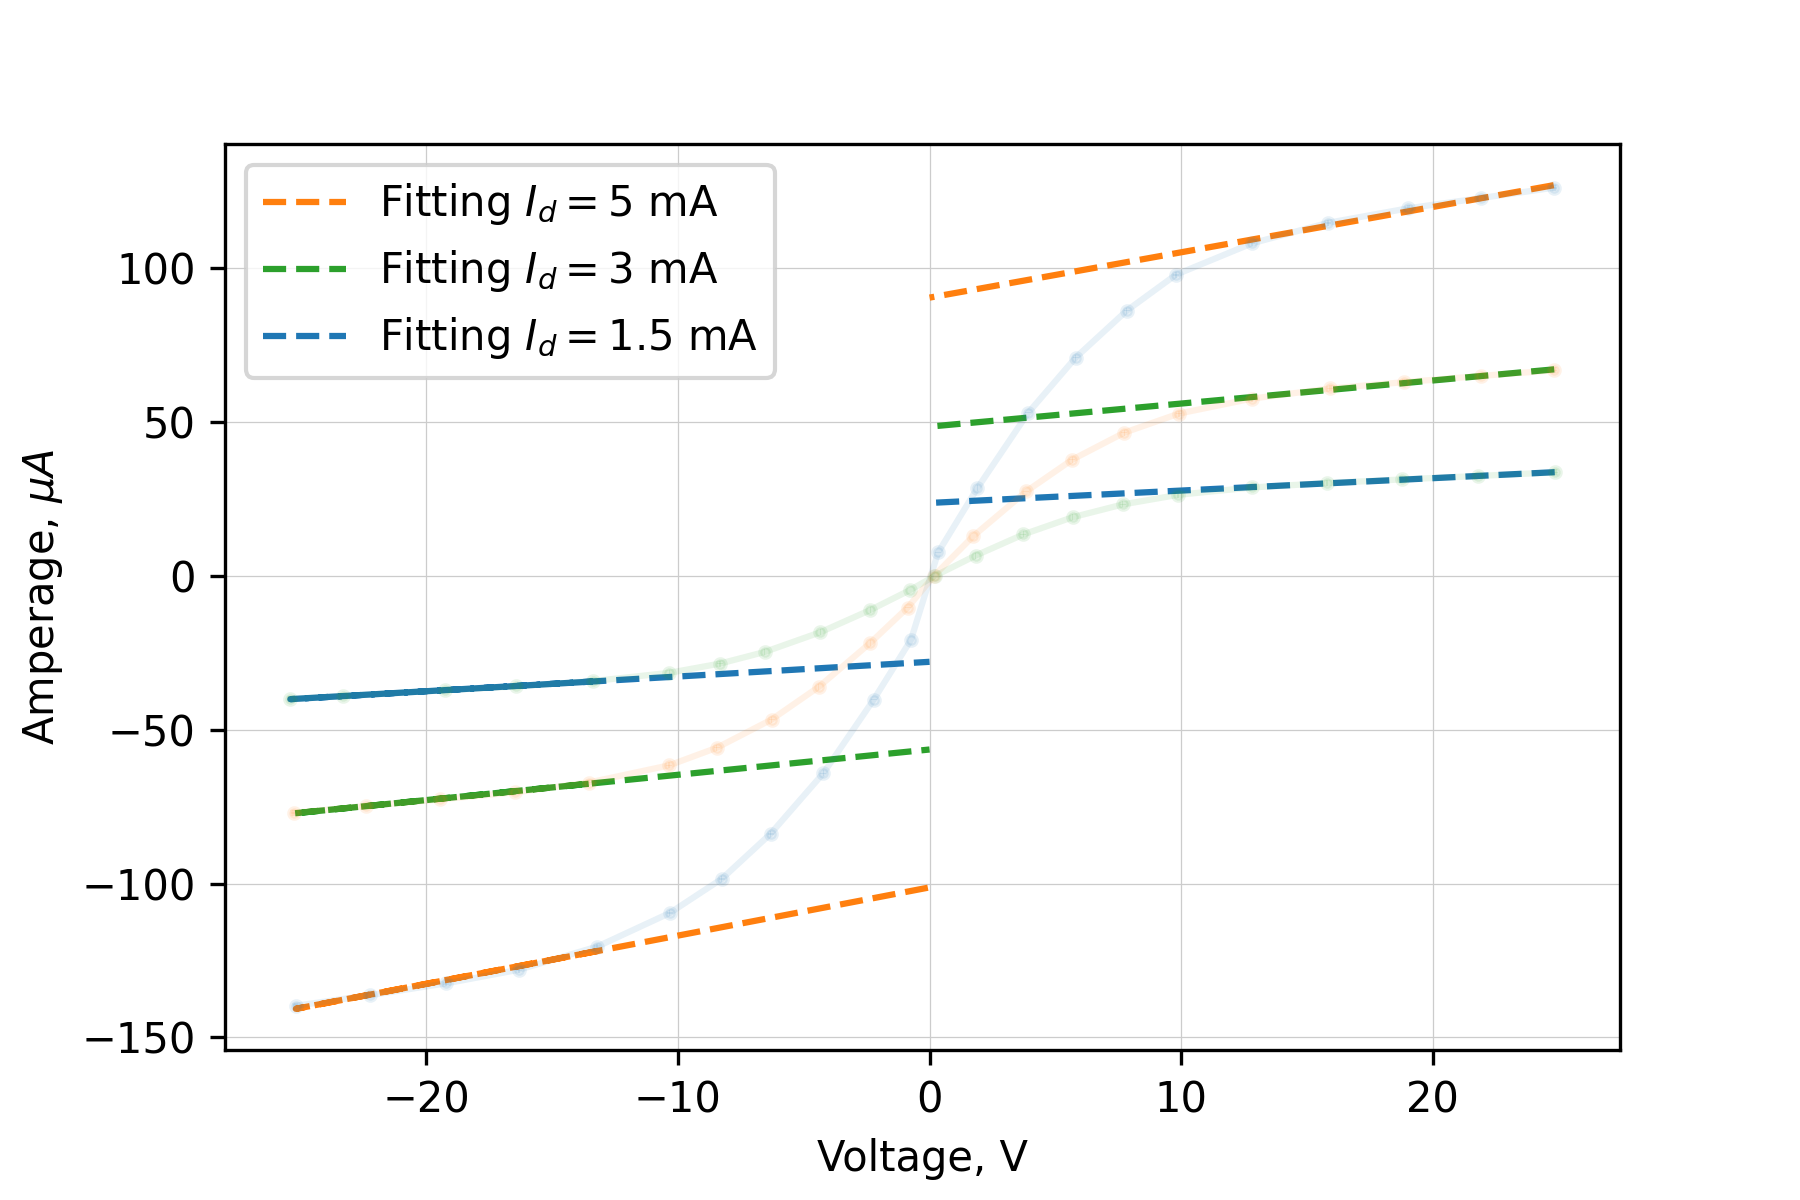
\includegraphics[height=\imageheight]{images/vah-probe.png}
    \caption{ВАХ двойного зонда}
    \label{fig:my_label}
\end{figure}

\newpage
Определим асимптоты:

\begin{figure}
    \centering
    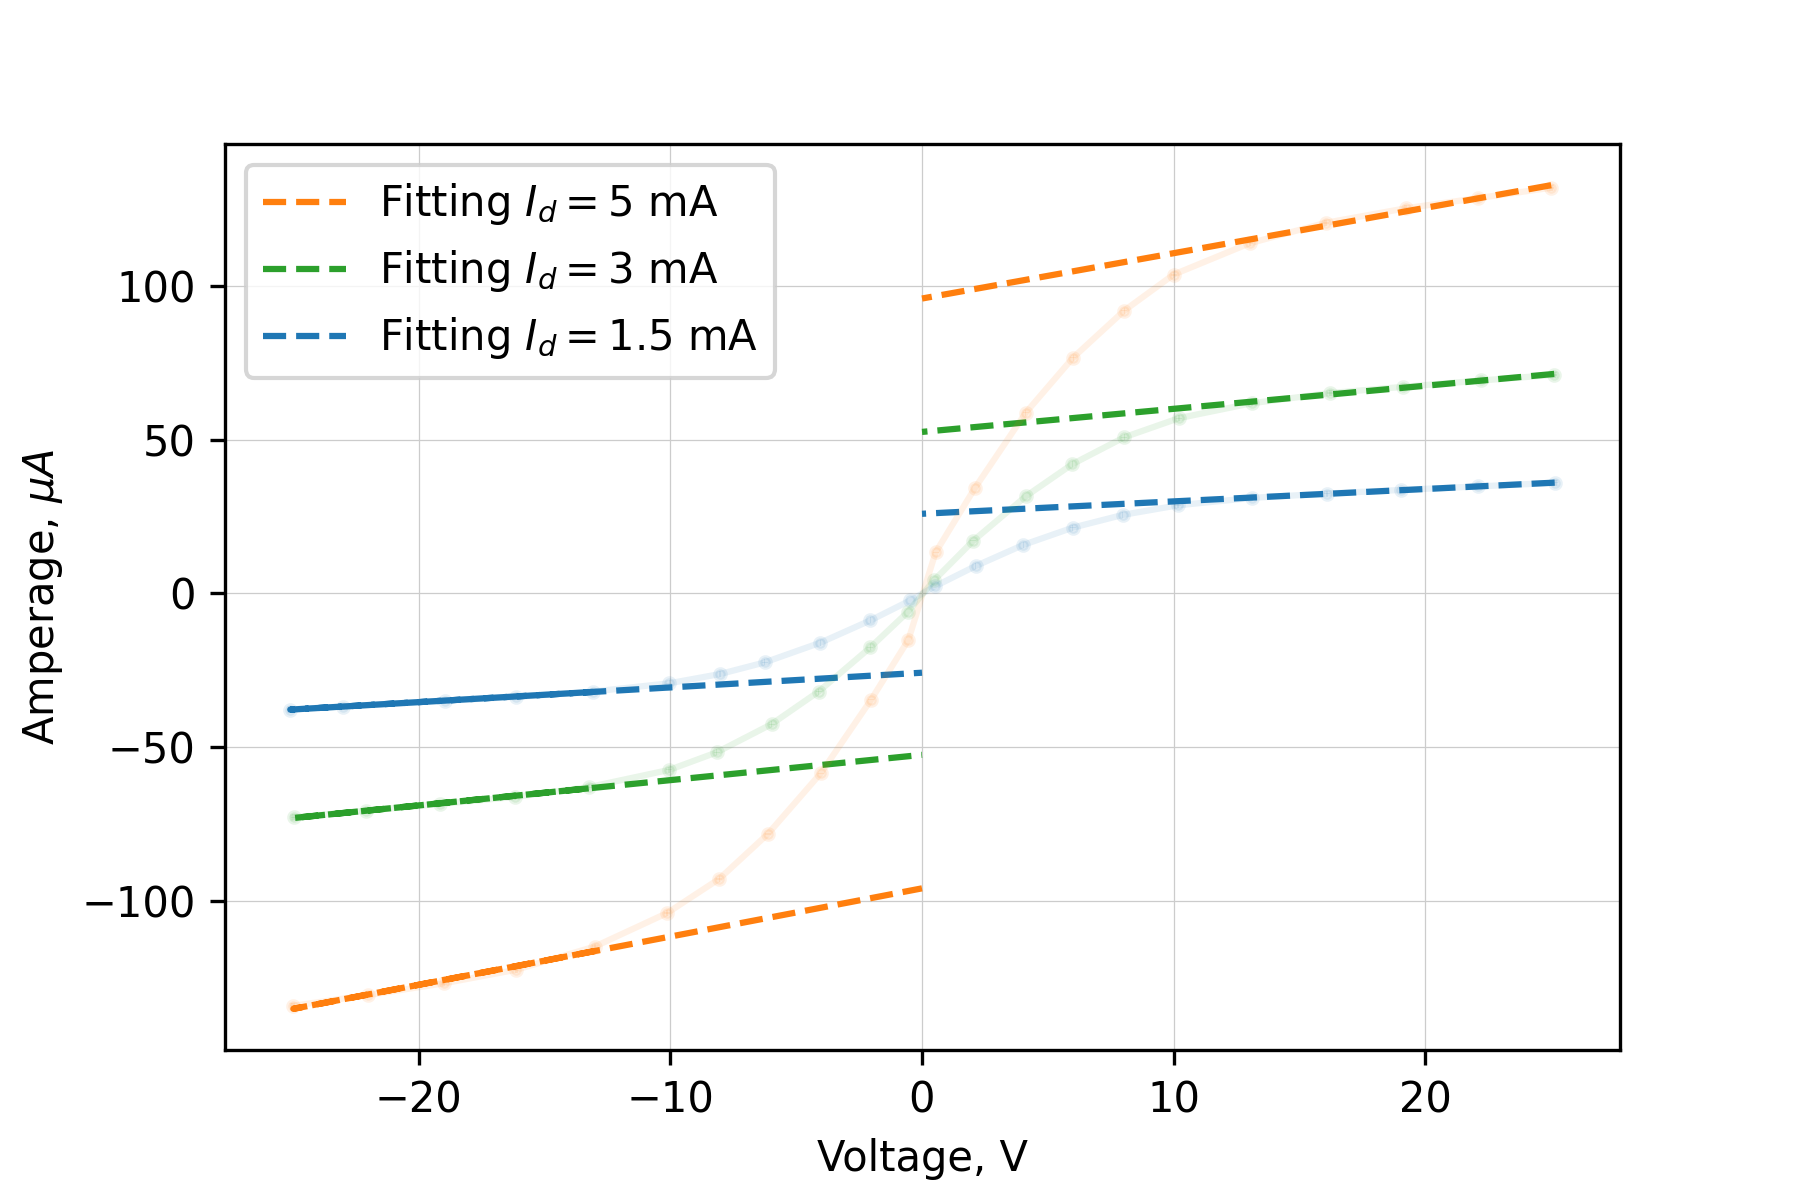
\includegraphics{images/vah-probe-fit.png}
    \caption{Асимптоты ВАХ зондов}
    \label{fig:my_label}
\end{figure}

И по точкам пересечения асимптот с осью ординат найдём ионный ток насыщения:

\[I_{i\text{н}}^{5\text{В}}     = 95.8 \pm 0.5 \text{ мкА},\]
\[I_{i\text{н}}^{3\text{В}}     = 52.5 \pm 0.2 \text{ мкА},\]
\[I_{i\text{н}}^{1.5\text{В}}   = 25.9 \pm 0.1 \text{ мкА}.\]

Полученные данные занесём в таблицу:

\begin{table}[h!]
\centering
\begin{tabular}{|c|c|c|c|c|c|c|}
\hline
$I_p$, мА  & $T_e$, $10^4$ К   & $n_e$, $10^{15}$ м$^{-3}$ & $\omega_p$, $10^4$ рад/c & $r_D$, $10^{-5}$ см & $N_D$ & $\alpha$, $10^{-7}$ \\ \hline
5.0 & $41\pm 4$ & $58\pm 6$ & $144\pm 10$   & $49\pm 3$     & 30 & 24\\ \hline
3.0 & $42\pm 4$ & $33\pm 4$ & $107\pm 9$    & $66\pm 5$     & 40 & 13\\ \hline
1.5 & $41\pm 6$ & $16\pm 2$ & $75\pm 8$     & $94 \pm 10$   & 57 & 7\\ \hline
\end{tabular}
\end{table}

\section{Выводы}
Исследовав ВАХ разряда, мы пришли к выводу, что плазма находилась в состоянии \textit{поднормального тлеющего заряда}.

При исследовании зондовых характеристик удалось выяснить, что плазма \textit{идеальна} и \textit{квазинейтральна.}



\end{document}